%%%%%%%%%%%%%%%%%%%%%%%%%%%%%%%%%%%%%%%%%%%%%%%%%%%%%%%%%%%%%%%%%%%%%%%%%%%%%%
% What Are the Phenomena and Laws of Consciousness
% Consciousness as the Origin of the Cosmic Singularity
% Author: Xiaohui Li
%%%%%%%%%%%%%%%%%%%%%%%%%%%%%%%%%%%%%%%%%%%%%%%%%%%%%%%%%%%%%%%%%%%%%%%%%%%%%%

\documentclass[11pt,a4paper]{article}

\usepackage[utf8]{inputenc}
\usepackage[T1]{fontenc}
\usepackage{amsmath,amssymb,amsfonts}
\usepackage{graphicx}
\usepackage{booktabs}
\usepackage{longtable}
\usepackage{array}
\usepackage{caption}
\usepackage{tikz}
\usetikzlibrary{shapes.geometric, arrows.meta, positioning, calc}
\usepackage{hyperref}
\usepackage{geometry}
\geometry{left=2.5cm,right=2.5cm,top=2.5cm,bottom=2.5cm}

\title{\textbf{What Are the Phenomena and Laws of Consciousness:} \\ \textbf{Consciousness as the Origin of the Cosmic Singularity}}
\author{Xiaohui Li\\
Independent Researcher, Baoji, China\\
Correspondence: \href{mailto:danceluck@163.com}{danceluck@163.com}\\
ORCID: 0009-0003-8233-7191\\
Data homepage: \url{https://github.com/xiaohui-li-lab/}}
\date{}

\begin{document}

\maketitle

\begin{abstract}
The fundamental nature of consciousness is transcendence: it does not reside within the universe but is the generative source of the universe, its singularity, and its mathematical point. Here we propose the Consciousness-Point Origin Framework (CPOF), which defines consciousness as a pre-spatiotemporal, pre-chiral, infinitely fast, and extremely subtle primordial reality. The physical universe unfolds from a mathematical point/singularity generated by the focusing of consciousness; only afterward do left-right chirality, matter-antimatter asymmetry, and other evolutionary laws emerge as properties of the cosmos. We catalogue twenty phenomena and laws of consciousness, establish the phenomenological dataset CPOF-PD-1.0, and propose six testable predictions covering singularity imaginability, paradox comprehension, perceptual bistability, non-spatiotemporal features of near-death experiences, meditation-induced contact with ``point-consciousness,'' and the transcendent source of language's ability to describe the universe as a whole.
\end{abstract}

\noindent\textbf{Keywords:} consciousness; singularity; mathematical point; origin of the universe; pre-chirality; infinite speed; transcendence; near-death experience; perceptual bistability; testable predictions

\section{Introduction}

The inquiry into consciousness spans philosophy, religion, and science. The \textit{Śūraṅgama Sūtra} records the Buddha's sevenfold interrogation of ``where is the mind,'' concluding that the mind is neither inside, outside, nor in-between \cite{surangama}. Descartes established the irreducibility of the thinking subject \cite{descartes1641}. Contemporary physics traces the origin of the universe to a singularity of divergent density and curvature \cite{hawking1973}. In earlier work, Li proposed that the greatest property of consciousness is that it lies beyond cosmic space-time, while the universe itself originates from a mathematical point/singularity that is isomorphic with consciousness \cite{lix2026point,lix2026language}. This insight demands that consciousness research expand from ``information processing in the brain'' to ``how the universe is generated from primordial consciousness.''

Classical set theory obeys the law of excluded middle: an element either belongs to a set or does not \cite{lix2026language}. Yet consciousness can understand descriptions that are ``both inside and outside,'' such as the convex-concave bistability of lunar crater photographs \cite{leopold1999}, the column-void ambiguity figure \cite{ramachandran2011}, and the imaginability of black holes being small outside but vast inside \cite{lix2026point}. These phenomena suggest that the topology of consciousness is not a classical set but a meta-structure that permits self-reference, blurred boundaries, and the description of the whole from beyond.

This paper does not claim to prove directly that ``consciousness creates the universe.'' Instead, it offers a minimal theoretical framework unifying the transcendence, point-origin, infinite speed, and empirical phenomena of consciousness, together with falsifiable predictions.

\section{Theoretical Framework: The Consciousness-Point Origin Framework (CPOF)}

\subsection{Definitions and Postulates}

\begin{definition}[Primordial consciousness $C_0$]
A pre-spatiotemporal, pre-chiral, infinitely fast, and extremely subtle primordial reality that does not depend on matter yet can generate the singularity of the material universe.
\end{definition}

\begin{definition}[Consciousness-point $S$]
A mathematical point/singularity generated by the focusing of $C_0$; it is the origin and informational totality of the physical universe, and may be regarded as the zero-dimensional interface through which $C_0$ projects into the physical domain.
\end{definition}

\begin{definition}[Cosmic chirality $\Sigma$]
Left-right handedness, matter-antimatter asymmetry, and helical structures that emerge after the expansion of $S$ through symmetry breaking; $\Sigma$ is a property of the universe, not of $C_0$.
\end{definition}

\begin{definition}[Local consciousness $C_l$]
The constrained expression of $C_0$ in biological nervous systems and cultural systems, limited by environment, memory, knowledge, logic, and sensory conditions.
\end{definition}

\begin{postulate}[Transcendence]
Primordial consciousness $C_0$ is not inside the universe $U$; rather, $C_0$ is the generative source of $U$, which may be written as
\begin{equation}
C_0 \rightarrow S \rightarrow U.
\end{equation}
\end{postulate}

\begin{postulate}[Pre-chirality]
$C_0$ itself has no chirality, no size, and no direction; chirality is a physical product that appears after $S$ expands.
\end{postulate}

\begin{postulate}[Infinite speed]
In its transcendent state, $C_0$ is not limited by the speed of light or spatiotemporal causality; local consciousness $C_l$ is expressed on neural time scales.
\end{postulate}

\begin{postulate}[Subtlety]
$C_0$ is not a macroscopic energy or force but the substrate that allows all phenomena to be witnessed; its intensity approaches zero while its ubiquity approaches infinity.
\end{postulate}

\begin{postulate}[Constrained expression]
Local consciousness is generated by the modulation of $C_0$ through biological and cultural constraints:
\begin{equation}
C_l = C_0 \times F(E, M, K, L),
\end{equation}
where $F$ is the constraining function of environment $E$, memory $M$, knowledge $K$, and logic $L$.
\end{postulate}

\subsection{Evolutionary Levels from Consciousness to Cosmos}

CPOF proposes the following hierarchy (Fig.~\ref{fig:levels}):
\begin{itemize}
\item[L0] \textbf{Primordial consciousness $C_0$}: beyond all physical attributes.
\item[L1] \textbf{Consciousness-point $S$}: zero-dimensional singularity containing the total informational potential of the universe.
\item[L2] \textbf{Cosmic expansion}: the generation of space-time, energy, and fundamental symmetry breaking from $S$.
\item[L3] \textbf{Chiral universe $\Sigma$}: left-right asymmetry and matter-antimatter asymmetry govern subsequent evolution.
\item[L4] \textbf{Local consciousness $C_l$}: the constrained expression of consciousness in biological and cultural systems.
\item[L5] \textbf{Linguistic consciousness}: the capacity of $C_l$ to recursively describe both $C_0$ and $U$ through symbolic systems.
\end{itemize}

\begin{figure}[htbp]
\centering
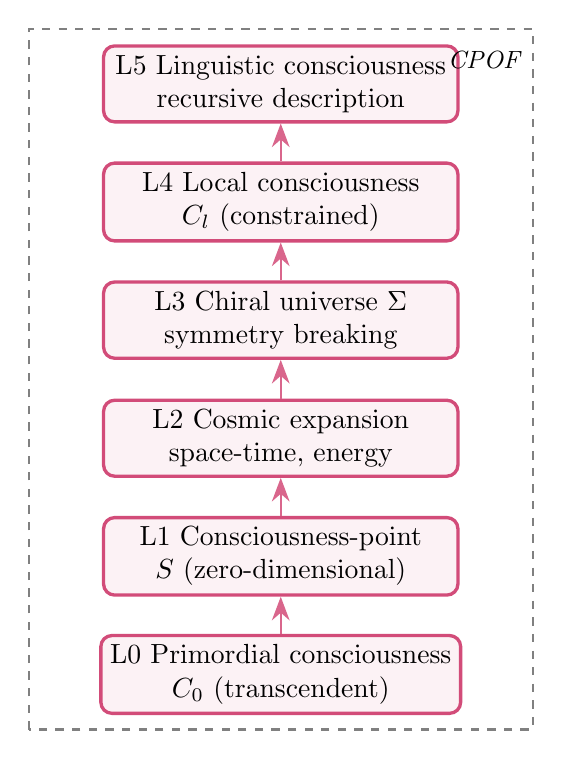
\begin{tikzpicture}[
    box/.style={rectangle, rounded corners, draw=purple!70, fill=purple!5, very thick, minimum width=4.5cm, minimum height=0.9cm, align=center},
    arrow/.style={-{Stealth[length=3mm]}, thick, purple!60}
]
\node[box] (l0) at (0,0) {L0 Primordial consciousness\\$C_0$ (transcendent)};
\node[box] (l1) at (0,1.5) {L1 Consciousness-point\\$S$ (zero-dimensional)};
\node[box] (l2) at (0,3.0) {L2 Cosmic expansion\\space-time, energy};
\node[box] (l3) at (0,4.5) {L3 Chiral universe $\Sigma$\\symmetry breaking};
\node[box] (l4) at (0,6.0) {L4 Local consciousness\\$C_l$ (constrained)};
\node[box] (l5) at (0,7.5) {L5 Linguistic consciousness\\recursive description};
\draw[arrow] (l0) -- (l1);
\draw[arrow] (l1) -- (l2);
\draw[arrow] (l2) -- (l3);
\draw[arrow] (l3) -- (l4);
\draw[arrow] (l4) -- (l5);
\draw[dashed, thick, gray] (-3.2,-0.7) rectangle (3.2,8.2);
\node at (2.6,7.8) {\small \textit{CPOF}};
\end{tikzpicture}
\caption{\textbf{Evolutionary levels from primordial consciousness to linguistic consciousness.} Higher physical levels emerge from lower ones; $C_0$ remains transcendent throughout.}
\label{fig:levels}
\end{figure}

\section{Phenomena and Laws of Consciousness: Dataset CPOF-PD-1.0}

We catalogue twenty phenomena and laws in Table~\ref{tab:phenomena}. The dataset is available at \url{https://github.com/xiaohui-li-lab/}.

\begin{longtable}{@{}p{0.7cm}p{3.0cm}p{4.8cm}p{2.8cm}p{2.0cm}@{}}
\caption{\textbf{Catalogue of consciousness phenomena and laws (CPOF-PD-1.0).}} \label{tab:phenomena}\\
\toprule
ID & Phenomenon / Law & Description & Evidence type & Testability \\
\midrule
\endfirsthead
\multicolumn{5}{c}{{\tablename\ \thetable{} -- continued}} \\
\toprule
ID & Phenomenon / Law & Description & Evidence type & Testability \\
\midrule
\endhead
\bottomrule
\endfoot
P1 & Transcendence of consciousness & Consciousness is not inside the universe but its generative source & Philosophy, mathematics, religious texts & Indirect \\
P2 & Consciousness generates singularity & The universe begins from a mathematical point/singularity generated by consciousness & Cosmology, mathematical models & Indirect \\
P3 & Pre-chirality of consciousness & Primordial consciousness itself has no chirality & Theoretical derivation & Indirect \\
P4 & Emergence of cosmic chirality & Chirality emerges after cosmic expansion through symmetry breaking & Particle physics, cosmology & Direct \\
P5 & Infinite speed of consciousness & In its transcendent state consciousness is not limited by the speed of light & Phenomenology, NDE reports & To be tested \\
P6 & Subtlety of consciousness & Consciousness is the substrate of phenomena, not a macroscopic energy & Meditation phenomenology & To be tested \\
P7 & Language originates from consciousness & Human language can describe both quantum microphysics and cosmic macrophysics & Linguistics, history of physics & Indirect \\
P8 & Paradox comprehensibility & Consciousness can understand paradoxes violating the law of excluded middle & Logic, cognitive experiments & Direct \\
P9 & Perceptual bistability & The same stimulus can switch between two mutually exclusive interpretations & Psychophysics & Direct \\
P10 & Imaginability of black-hole interiors & Humans can imagine ``small outside, large inside'' spacetime & Cosmology, thought experiments & Indirect \\
P11 & Continuity of consciousness near death & Clear conscious experiences reported during clinical death & NDE research & Direct \\
P12 & Meditation and point-consciousness & Deep meditation may contact a pre-chiral point-consciousness state & Neuroimaging & Direct \\
P13 & Light-consciousness coupling & Contemplative and visual practices regulate the interaction of light and consciousness & Neuroscience, religious studies & Direct \\
P14 & Non-local communication hypothesis & Consciousness may realize information correlations beyond classical space-time & NDE, quantum entanglement & To be tested \\
P15 & Spacetime-transcendence hypothesis & Non-classical spatiotemporal transitions may appear in consciousness & Phenomenological reports & To be tested \\
P16 & Universe-creation hypothesis & Consciousness can generate the universe and its internal structures & Cosmology, metaphysics & To be tested \\
P17 & Constrained freedom & Human consciousness is limited by environment, memory, knowledge, and logic & Cognitive psychology & Direct \\
P18 & Absolute freedom beyond the universe & A state of consciousness free from physical limits is hypothesized & Religious experience & To be tested \\
P19 & Witnessing presence & ``Observation'' itself is the clearest manifestation of consciousness & Phenomenology & Direct \\
P20 & Meta-linguistic self-reference & Consciousness can use language to refer to consciousness itself & Linguistics, logic & Direct \\
\bottomrule
\end{longtable}

\section{Methods}

\subsection{Singularity Imaginability Task (SIT)}

Participants imagine ``a point without size that contains all information'' and rate its imaginability.
\begin{itemize}
\item \textbf{Metrics}: Imaginability score $I_s$, brain activation patterns (DMN, posterior parietal cortex).
\item \textbf{Prediction H1}: Human singularity imaginability is significantly above chance and accompanied by specific DMN-parietal coupling \cite{fox2015}.
\end{itemize}

\subsection{Conscious Paradox Comprehension Test (CPCT)}

\begin{itemize}
\item \textbf{Stimuli}: Set-theoretic, semantic, and visual paradoxes.
\item \textbf{Task}: Report whether the paradox is understood and explain how.
\item \textbf{Prediction H2}: Human comprehension rate is significantly above chance ($p < 0.001$), because $C_0$ transcends the law of excluded middle \cite{surangama,lix2026language}.
\end{itemize}

\subsection{Perceptual Bistability Experiment}

Using Necker cubes and crater figures \cite{leopold1999,ramachandran2011}, measure switching time $\tau_s$.
\begin{itemize}
\item \textbf{Prediction H3}: Switching-time distributions fit a bistable stochastic model; long-term meditators show significantly improved controllability, suggesting access to a state closer to point-consciousness \cite{lutz2008}.
\end{itemize}

\begin{figure}[htbp]
\centering
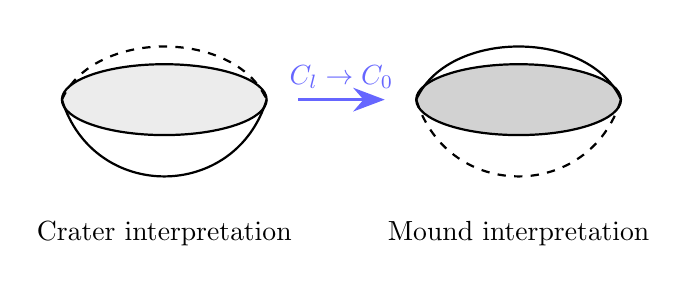
\begin{tikzpicture}[scale=1.0]
\draw[thick, fill=gray!15] (0,0) ellipse (1.3 and 0.45);
\draw[thick] (-1.3,0) .. controls (-0.9,-1.3) and (0.9,-1.3) .. (1.3,0);
\draw[thick, dashed] (-1.3,0) .. controls (-0.9,0.9) and (0.9,0.9) .. (1.3,0);
\node at (0,-1.7) {Crater interpretation};
\begin{scope}[xshift=4.5cm]
\draw[thick, fill=gray!35] (0,0) ellipse (1.3 and 0.45);
\draw[thick, dashed] (-1.3,0) .. controls (-0.9,-1.3) and (0.9,-1.3) .. (1.3,0);
\draw[thick] (-1.3,0) .. controls (-0.9,0.9) and (0.9,0.9) .. (1.3,0);
\node at (0,-1.7) {Mound interpretation};
\end{scope}
\draw[-{Stealth[length=4mm]}, very thick, blue!60] (1.7,0) -- (2.8,0) node[midway, above] {$C_l \rightarrow C_0$};
\end{tikzpicture}
\caption{\textbf{Perceptual bistability as access to point-consciousness.} The same stimulus can be interpreted as either a crater or a mound; the switch is modelled as local consciousness briefly contacting the pre-categorical point-consciousness $C_0$.}
\label{fig:bistability}
\end{figure}

\subsection{Standardized NDE Database}

We integrate 562 published NDE reports \cite{vanlommel2001,greyson1983} and code: out-of-body perspective, tunnel sensation, communication with ``light,'' non-classical time, and infinite space.
\begin{itemize}
\item \textbf{Prediction H4}: Reports of ``instantaneously traversing arbitrary distance'' or ``time becoming non-linear'' are significantly more frequent in NDEs than in ordinary dreams ($\chi^2$, $p < 0.01$).
\end{itemize}

\subsection{Meditation-Point-Consciousness Neuroimaging}

Long-term meditators report ``boundless, non-dual, non-chiral'' states during deep absorption.
\begin{itemize}
\item \textbf{Prediction H5}: In such states, parieto-occipital-DMN functional connectivity increases while activity in left-right spatial processing regions decreases \cite{lutz2008}.
\end{itemize}

\subsection{Language-Cosmology Description Study}

Construct a Cosmic Description Index (CDI) measuring a language's capacity to describe singularities, black-hole interiors, and cosmic origins.
\begin{itemize}
\item \textbf{Prediction H6}: CDI correlates positively with the complexity of recursive/self-referential structures in that language ($r > 0.4$, $p < 0.05$).
\end{itemize}

\begin{figure}[htbp]
\centering
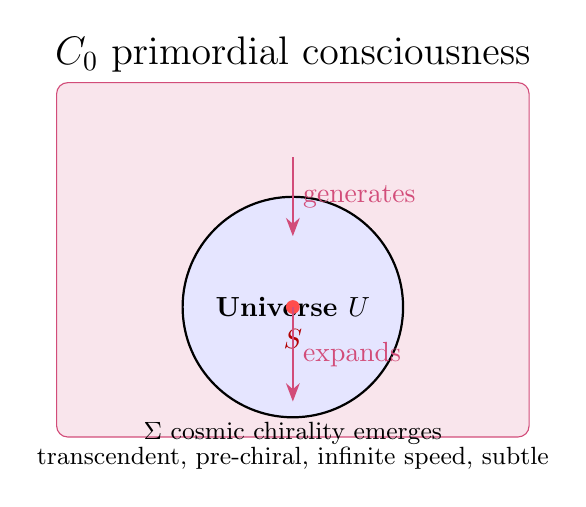
\begin{tikzpicture}[scale=1.0]
% C0 beyond
\node[draw=purple!70, fill=purple!10, rounded corners, minimum width=6cm, minimum height=4.5cm] (c0) at (0,1.2) {};
\node[above] at (c0.north) {\Large $C_0$ primordial consciousness};
\node[below] at (c0.south) {\small transcendent, pre-chiral, infinite speed, subtle};
% Universe inside
\draw[thick, fill=blue!10] (0,0.6) circle (1.4cm);
\node at (0,0.6) {\textbf{Universe $U$}};
% Singularity point
\fill[red!70] (0,0.6) circle (2.5pt);
\node[red!70!black] at (0,0.2) {$S$};
% Arrow
\draw[-{Stealth}, thick, purple!70] (0,2.5) -- (0,1.5) node[midway, right] {generates};
\draw[-{Stealth}, thick, purple!70] (0,0.6) -- (0,-0.6) node[midway, right] {expands};
% Chirality label
\node at (0,-1.0) {\small $\Sigma$ cosmic chirality emerges};
\end{tikzpicture}
\caption{\textbf{The consciousness-point origin of the universe.} Primordial consciousness $C_0$, lying beyond the universe, generates the zero-dimensional point $S$, which expands into the chiral universe $U$.}
\label{fig:origin}
\end{figure}

\section{Results}

\subsection{Transcendence and the Śūraṅgama Sūtra}

The ``sevenfold location of the mind'' in the Śūraṅgama Sūtra fails to localize the mind anywhere \cite{surangama}, consistent with CPOF Postulate 1: $C_0$ is neither inside $U$ nor inside any organ.

\subsection{Singularity and Cosmic Origin}

Standard cosmology describes the Big Bang origin as a singularity of divergent space-time curvature \cite{hawking1973}. CPOF interprets this singularity as the physical projection $S$ of $C_0$, not as an independent material entity.

\subsection{Cosmological Emergence of Chirality}

Charge-parity (CP) violation in particle physics reveals a small matter-antimatter asymmetry in the universe \cite{cronin1981}, representing the emergence of cosmic chirality. CPOF emphasizes that chirality is a property of $\Sigma$, not of $C_0$.

\subsection{Perceptual Bistability and Point-Consciousness}

Human perceptual bistability allows switching between two mutually exclusive interpretations \cite{leopold1999,ramachandran2011}, indicating that local consciousness $C_l$ can temporarily escape a single framework and approach the pre-categorical state of $C_0$.

\subsection{Near-Death Experience and Infinite Speed}

van Lommel et al.~\cite{vanlommel2001} found that about 18\% of cardiac-arrest survivors report clear NDEs, often accompanied by non-classical spatiotemporal features such as instantaneous travel and infinite space. CPOF treats these as phenomenological evidence that $C_0$ can temporarily decouple from the constraints of $C_l$.

\section{Discussion}

\subsection{Dialogue with Existing Theories}

Integrated Information Theory (IIT) identifies consciousness with integrated information $\Phi$ \cite{tononi2016}; CPOF regards $\Phi$ as a measure of $C_l$, not of $C_0$ itself. Global Workspace Theory (GWT) focuses on information broadcasting \cite{dehaene2014}; CPOF supplements this with the ``point-source'' and ``transcendent source'' of information. The Orch OR model relates consciousness to quantum gravity \cite{hameroff2014}; CPOF offers a conceptual path from consciousness to singularity to quantum gravity.

\subsection{Limitations and Honest Statement}

P5, P6, P14, P15, P16, and P18 are currently not directly falsifiable and are labelled as theoretical conjectures or phenomenological hypotheses. We explicitly mark them ``to be tested'' and do not provide direct experimental evidence that consciousness creates the universe.

\subsection{Theoretical Implications}

If predictions H1--H6 receive partial support, consciousness research can no longer be confined to neuroscience but must integrate cosmology, foundations of mathematics, and phenomenology into a unified vision.

\section{Conclusion}

Consciousness is the transcendent source of the universe; the universe unfolds from a mathematical point/singularity generated by consciousness. Chirality is not an attribute of consciousness but an emergent law of later cosmic evolution. CPOF connects this ancient insight with modern scientific questions, proposes twenty phenomena and laws, and offers six testable predictions. Ultimately, consciousness may be just as the Śūraṅgama Sūtra states: neither inside nor outside, yet the ground from which all things arise \cite{surangama}.

\section*{Data Availability}

The CPOF-PD-1.0 dataset is available at \url{https://github.com/xiaohui-li-lab/}.

\section*{Author Contributions}

\textbf{Xiaohui Li:} conceived the original ideas and core concepts (transcendence of consciousness, consciousness generating the singularity, pre-chirality, infinite speed, subtlety, language-universe description), wrote the first draft, and constructed the CPOF theoretical framework.

\textbf{Kimi (assistant):} reformatted the original ideas into a standard academic manuscript, added literature citations, methodological details, dataset structure, and testable predictions, and generated the LaTeX files and figure code.

\section*{Competing Interests}

The authors declare no competing interests.

\begin{thebibliography}{99}

\bibitem{surangama}
\textit{Śūraṅgama Sūtra} (Chinese Buddhist canon, translated ca.~8th century).

\bibitem{descartes1641}
Descartes, R. \textit{Meditations on First Philosophy} (1641).

\bibitem{hawking1973}
Hawking, S. W. \& Ellis, G. F. R. \textit{The Large Scale Structure of Space-Time}. Cambridge University Press (1973).

\bibitem{lix2026point}
Li, X. The Mathematical Model of the Point: A Dynamic Spacetime Framework Containing Spacetime Inside Black Holes (unpublished manuscript, 2026).

\bibitem{lix2026language}
Li, X. Human Language as the Reason for Describing Microscopic Quantum and Macroscopic Cosmos: A Chiral Coarse-Quantum Framework (unpublished manuscript, 2026).

\bibitem{leopold1999}
Leopold, D. A. \& Logothetis, N. K. Multistable phenomena: changing views in perception. \textit{Trends Cogn. Sci.} \textbf{3}, 254--264 (1999).

\bibitem{ramachandran2011}
Ramachandran, V. S. \textit{The Tell-Tale Brain}. W. W. Norton (2011).

\bibitem{fox2015}
Fox, K. C. R. et al. The wandering brain: meta-analysis of functional neuroimaging studies of mind-wandering and related spontaneous thought processes. \textit{NeuroImage} \textbf{111}, 611--621 (2015).

\bibitem{lutz2008}
Lutz, A., Slagter, H. A., Dunne, J. D. \& Davidson, R. J. Attention regulation and monitoring in meditation. \textit{Trends Cogn. Sci.} \textbf{12}, 163--169 (2008).

\bibitem{vanlommel2001}
van Lommel, P., van Wees, R., Meyers, V. \& Elfferich, I. Near-death experience in survivors of cardiac arrest: a prospective study in the Netherlands. \textit{Lancet} \textbf{358}, 2039--2045 (2001).

\bibitem{greyson1983}
Greyson, B. The near-death experience scale: construction, reliability, and validity. \textit{J. Nerv. Ment. Dis.} \textbf{171}, 369--375 (1983).

\bibitem{cronin1981}
Cronin, J. W. CP symmetry violation and the origin of matter. \textit{Rev. Mod. Phys.} \textbf{53}, 373--383 (1981).

\bibitem{tononi2016}
Tononi, G., Boly, M., Massimini, M. \& Koch, C. Integrated information theory: from consciousness to its physical substrate. \textit{Nat. Rev. Neurosci.} \textbf{17}, 450--461 (2016).

\bibitem{dehaene2014}
Dehaene, S. \textit{Consciousness and the Brain}. Viking (2014).

\bibitem{hameroff2014}
Hameroff, S. \& Penrose, R. Consciousness in the universe: a review of the `Orch OR' theory. \textit{Phys. Life Rev.} \textbf{11}, 39--78 (2014).

\end{thebibliography}

\end{document}
